\documentclass[11pt]{amsart}

\usepackage{physics}
\usepackage{amsmath}
\usepackage{graphicx}

\renewcommand{\thesubsection}{\thesection.\alph{subsection}}

\title[Relativistic Kinematics]{Relativistic Kinematics \\
	\hrulefill \small{ FYS3120: Problem Set 8 } \hrulefill}

\author[Winther-Larsen]{Sebastian G. Winther-Larsen}

\date{\today}

\begin{document}

\maketitle

\section{Mirror Mirror on the (Moving) Wall}

A monocromatic light source is at rest in the laboratory and sends photons with frequency $\nu_0$ towards a mirror which has its reflective surface perpendicular to the beam direction. The mirror moves away from the light source with velocity $v$. The transformation formula for four-momentum is given by $p^{\mu} = (E/c, \vb{p})$ and the Planck relation is $E=h\nu$.

\subsection{Light Frequency in Rest Frame of Mirror}
The relativistic energy of a moving particle is 
\begin{equation}
E = \sqrt{p^2c^2 + m^2c^4}.
\end{equation}
Because a photon is without mass, the energy of a photon according to the formula above is
\begin{equation}
E = pc,
\end{equation}
which can be inserted into Planck relation yielding
\begin{equation}
p = \frac{h \nu_0}{c}.
\end{equation}
This provides an expression for the four vector
\begin{equation}
p^\mu = \left(\frac{E}{c}, \vb{p} \right) = \left(\frac{h\nu_0}{c} \right) = (p,p,0,0).
\end{equation} 
To get from emitted frequency $\nu_0$ in lab reference frame $S$, to frequency $\nu$ in mirror reference frame $S'$ one needs to take the Lorentz transform 
\begin{equation}
p'^\mu = L^\mu_{\ \rho} p^\rho,
\end{equation}
because the mirror reference frame is just a boost along the $x$-axis, relative to the lab reference frame.
\begin{equation}
\begin{pmatrix}
p'^0 \\ p'^1 \\ p'^2 \\ p'^3
\end{pmatrix}
=
\begin{pmatrix}
\gamma & -\beta\gamma & 0 & 0 \\
-\beta\gamma & \gamma & 0 & 0 \\
0 & 0 & 1 & 0 \\
0 & 0 & 0 & 1
\end{pmatrix}
\begin{pmatrix}
p^0 \\ p^1 \\ p^2 \\ p^3
\end{pmatrix}
=
\gamma(1-\beta)
\begin{pmatrix}
p \\ p \\ 0 \\ 0
\end{pmatrix},
\end{equation}
so
\begin{equation}
p' = \gamma(1-\beta)p.
\end{equation}
The de Broglie relations gives
\begin{equation}
p = \frac{h}{\lambda} = \frac{h\nu}{c},
\end{equation}
so the frequency of the emitted and reflected light in the rest frame of the mirror must be
\begin{equation}
\nu' = \gamma(1-\beta)\nu.
\end{equation}
The frequency of the emitted and reflected light must necessarily be the same, due to conservation of momentum.

\subsection{Frequency of Reflected Light in Lab System}

Denoting frequency of reflected light as $\nu_R$ and frequency of emitted light as $\nu_0$, we already have that
\begin{equation}
\label{eq:mirrorRF}
\nu'_R = \gamma(1-\beta)\nu_0,
\end{equation}
in the mirror rest frame. Similarly, the frequency of reflected light in laboratory rest frame is
\begin{equation}
\label{eq:labRF}
\nu_R = \gamma(1-\beta)\nu'_R.
\end{equation}
Inserting \ref{eq:mirrorRF} into \ref{eq:labRF} yields
\begin{equation}
\nu_R = \gamma^2(1-\beta)^2\nu_0 = \frac{(1-\beta)^2}{1-\beta^2}\nu_0 = \frac{(1-\beta)^2}{(1+\beta)(1-\beta)}\nu_0 = \frac{1-\beta}{1+\beta}\nu_0
\end{equation}

\section{Relativistic Collision}
\begin{figure}
\centering
	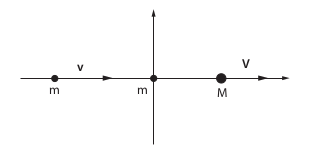
\includegraphics[width=0.8\textwidth]{collision.png}
	\caption{Collision between two particles of mass $m$ resulting in a particle with mass $M$}
	\label{fig:collision}
\end{figure}

Figure \ref{fig:collision} shows a particle with mass $m$ and (relativistic) kinetic energy $V$ in the laboratory frame $S$. The particles is moving towards another particle, with the same mass $m$, which is at rest in $S$.

\subsection{Velocity of First Particle}
Relativistic kinetic energy is given by
\begin{equation}
\label{eq:relkinenergy}
T = (\gamma-1)mc^2.
\end{equation}
Introducing the dimensionless quantity $\alpha = T/mc^2$,
\begin{align*}
\alpha = \frac{T}{mc^2} = \frac{(\gamma - 1)mc^2}{mc^2} &= (\gamma-1) = \frac{1}{\sqrt{1-\frac{v^2}{c^2}}} - 1 \\
\alpha + 1 &= \frac{1}{\sqrt{1-\beta^2}} \\
1 - \beta^2 &= \frac{1}{(\alpha + 1)^2} \\
\beta &= \pm \sqrt{1 - \frac{1}{(\alpha + 1)^2}} \\
v &= \pm c \sqrt{1-(\alpha + 1)^{-2}},
\end{align*}
yields an expression for the velocity of the moving particle.

\subsection{Compound Particle of Perfectly Inelastic Collision}
Assuming that the collision is completely inelastic, they will ``stick together'' after the collision, and form a new compounded particle. The momentum is conserved so that
\begin{equation}
\label{eq:momentumconservation1}
\left(\frac{E_1}{c}, \vb{p}_1 \right) + \left(\frac{E_2}{c}, \vb{p}_2 \right) = \left(\frac{E_3}{c}, \vb{p}_3 \right) ,
\end{equation}
where $E_1 = \gamma(v_1)mc^2$ and $E_2 = \gamma(v_2)mc^2$. Since $v_2 = 0$, $\gamma(v_2) = 1$ and $\vb{p}_2 = \vb{0}$. This gives a relation between the time elements of the four-momenta, which yields the energy of the compounded particle.
\begin{align}
\frac{E_1 + E_2}{c} &= \frac{E_3}{c} \nonumber \\
E_1 + E_2 &= E_3 \nonumber \\
R_3 =  \gamma mc^2 + mc^2 &= (1 + \gamma)mc^2.
\end{align}

Similarly, the momentum of the compounded particle must be
\begin{equation}
\vb{p}_3 = \vb{p}_1 = \gamma m\vb{v}_3 
\end{equation}



\end{document}